\documentclass[border=8pt]{standalone}
\usepackage{fontspec}
\setmainfont[
  Path = ../fonts/,
  UprightFont = Cabin-Regular.ttf,
  BoldFont = Cabin-Bold.ttf,
  ItalicFont = Cabin-Italic.ttf
]{Cabin}
\usepackage{amsmath, amssymb}
\usepackage{tikz}
\usetikzlibrary{arrows.meta, positioning, shapes.geometric, calc}

\begin{document}
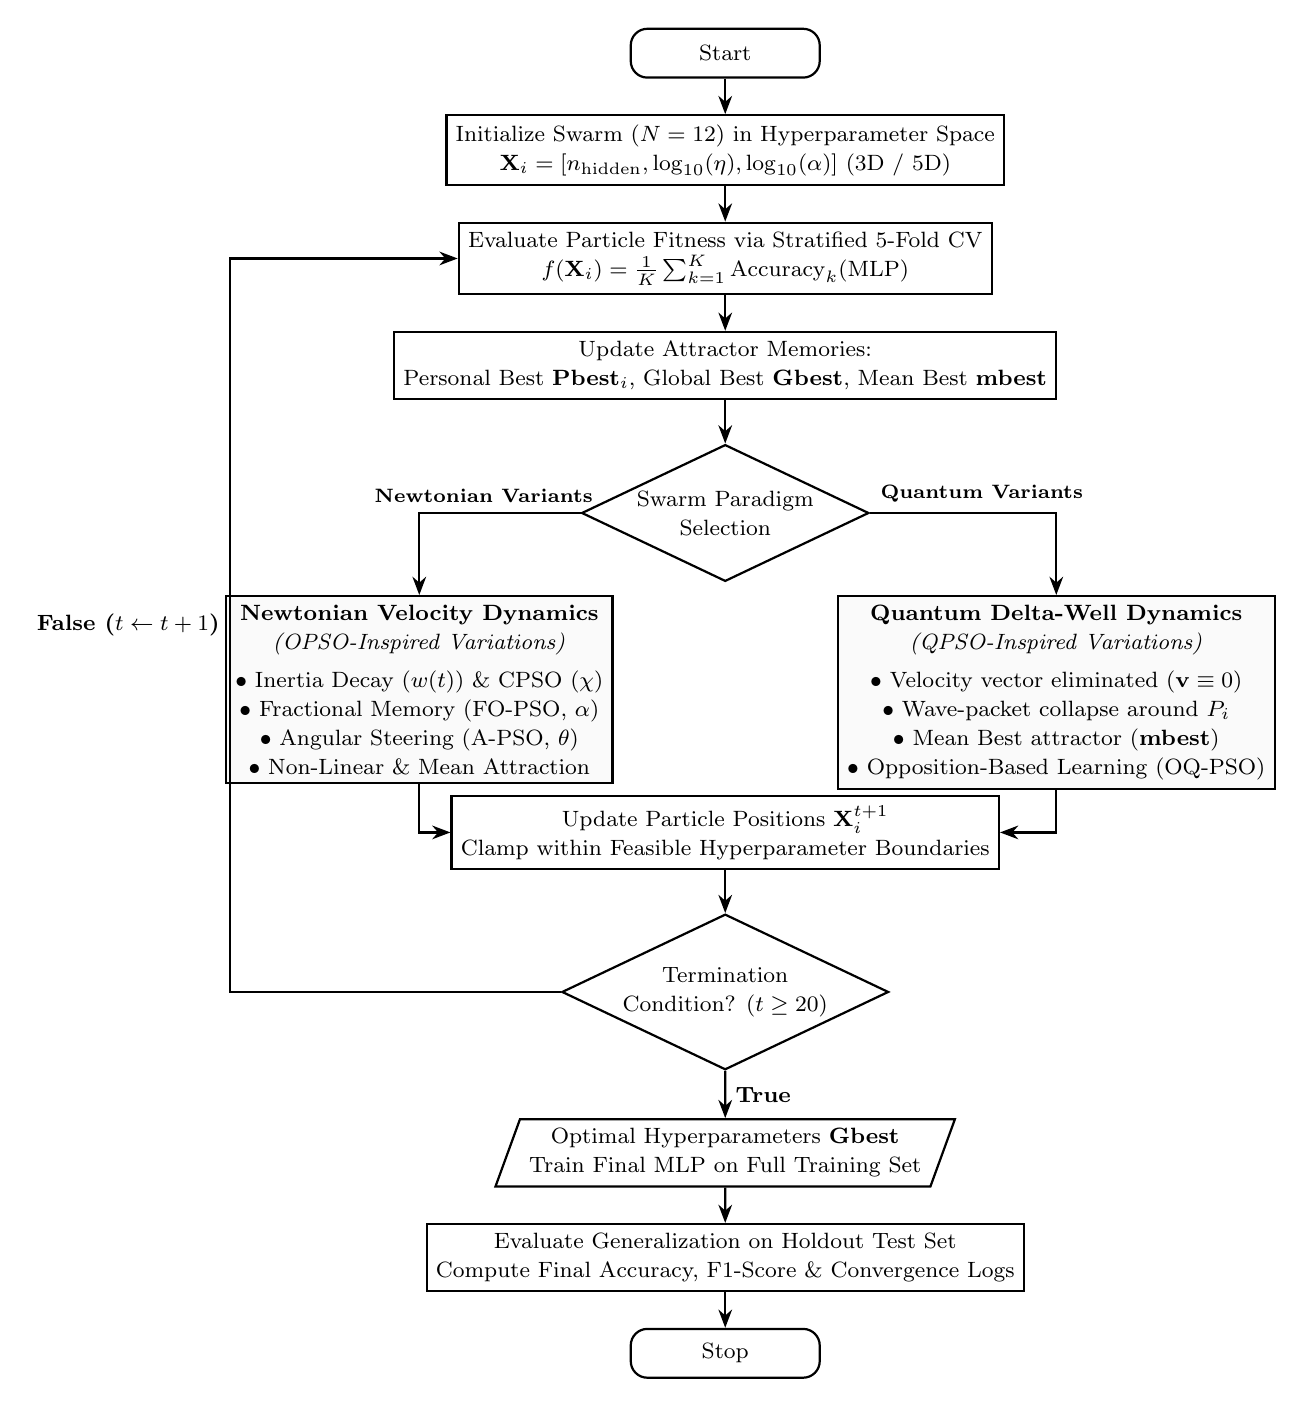
\begin{tikzpicture}[
    font=\fontsize{8pt}{10.5pt}\selectfont,
    >=Stealth,
    startstop/.style={draw, rounded corners=6pt, minimum width=2.4cm, minimum height=0.62cm, align=center, line width=0.8pt},
    process/.style={draw, rectangle, minimum width=4.0cm, minimum height=0.68cm, align=center, line width=0.8pt},
    subproc/.style={draw, rectangle, minimum width=3.4cm, minimum height=1.35cm, align=center, line width=0.75pt, fill=black!2},
    decision/.style={draw, diamond, aspect=2.1, minimum width=2.6cm, minimum height=0.8cm, align=center, line width=0.8pt, inner sep=1pt},
    data/.style={draw, trapezium, trapezium left angle=70, trapezium right angle=110, minimum width=3.2cm, minimum height=0.68cm, align=center, line width=0.8pt}
]

% Top Flow
\node (start) [startstop] {Start};
\node (init) [process, below=0.45cm of start] {Initialize Swarm ($N=12$) in Hyperparameter Space\\$\mathbf{X}_i = [n_{\mathrm{hidden}}, \log_{10}(\eta), \log_{10}(\alpha)]$ (3D / 5D)};
\node (eval) [process, below=0.45cm of init] {Evaluate Particle Fitness via Stratified 5-Fold CV\\$f(\mathbf{X}_i) = \frac{1}{K}\sum_{k=1}^K \mathrm{Accuracy}_k(\mathrm{MLP})$};
\node (update_best) [process, below=0.45cm of eval] {Update Attractor Memories:\\Personal Best $\mathbf{Pbest}_i$, Global Best $\mathbf{Gbest}$, Mean Best $\mathbf{mbest}$};

% Branching Split Node
\node (branch) [decision, below=0.55cm of update_best] {Swarm Paradigm\\Selection};

% Two Parallel Branches: Newtonian vs Quantum
\node (newton) [subproc, below left=0.6cm and 0.5cm of branch] {
    \textbf{Newtonian Velocity Dynamics}\\
    \textit{(OPSO-Inspired Variations)}\\[3pt]
    $\bullet$ Inertia Decay ($w(t)$) \& CPSO ($\chi$)\\
    $\bullet$ Fractional Memory (FO-PSO, $\alpha$)\\
    $\bullet$ Angular Steering (A-PSO, $\theta$)\\
    $\bullet$ Non-Linear \& Mean Attraction
};

\node (quantum) [subproc, below right=0.6cm and 0.5cm of branch] {
    \textbf{Quantum Delta-Well Dynamics}\\
    \textit{(QPSO-Inspired Variations)}\\[3pt]
    $\bullet$ Velocity vector eliminated ($\mathbf{v} \equiv 0$)\\
    $\bullet$ Wave-packet collapse around $P_i$\\
    $\bullet$ Mean Best attractor ($\mathbf{mbest}$)\\
    $\bullet$ Opposition-Based Learning (OQ-PSO)
};

% Merge Node
\node (merge) [process, below=2.7cm of branch] {Update Particle Positions $\mathbf{X}_i^{t+1}$\\Clamp within Feasible Hyperparameter Boundaries};

% Termination Check
\node (term) [decision, below=0.55cm of merge] {Termination\\Condition? ($t \ge 20$)};

% Bottom Flow
\node (opt) [data, below=0.6cm of term] {Optimal Hyperparameters $\mathbf{Gbest}$\\Train Final MLP on Full Training Set};
\node (test) [process, below=0.45cm of opt] {Evaluate Generalization on Holdout Test Set\\Compute Final Accuracy, F1-Score \& Convergence Logs};
\node (stop) [startstop, below=0.45cm of test] {Stop};

% Connections Top
\draw[->, line width=0.8pt] (start) -- (init);
\draw[->, line width=0.8pt] (init) -- (eval);
\draw[->, line width=0.8pt] (eval) -- (update_best);
\draw[->, line width=0.8pt] (update_best) -- (branch);

% Branching Connections
\draw[->, line width=0.8pt] (branch.west) -| node[above, font=\scriptsize\bfseries, pos=0.3] {Newtonian Variants} (newton.north);
\draw[->, line width=0.8pt] (branch.east) -| node[above, font=\scriptsize\bfseries, pos=0.3] {Quantum Variants} (quantum.north);

% Merging Connections
\draw[->, line width=0.8pt] (newton.south) |- (merge.west);
\draw[->, line width=0.8pt] (quantum.south) |- (merge.east);

% Loop & Termination
\draw[->, line width=0.8pt] (merge) -- (term);
\draw[->, line width=0.8pt] (term) -- node[right, font=\footnotesize\bfseries] {True} (opt);
\draw[->, line width=0.8pt] (opt) -- (test);
\draw[->, line width=0.8pt] (test) -- (stop);

% False Loop Back
\draw[->, line width=0.8pt] (term.west) -- ++(-4.2,0) |- node[near start, left, font=\footnotesize\bfseries] {False ($t \leftarrow t+1$)} (eval.west);

\end{tikzpicture}
\end{document}
